% Harus dimuat terlebih dahulu, digunakan agar file PDF memiliki format karakter yang benar.
% Untuk informasi lebih lanjut, lihat https://ctan.org/pkg/cmap.
\RequirePackage{cmap}

% Format dokumen sebagai paper konferensi menggunakan aturan IEEEtran terbaru (v1.8b).
% Untuk informasi lebih lanjut, lihat http://www.michaelshell.org/tex/ieeetran/.
\documentclass[conference]{IEEEtran}[2015/08/26]

% Format encoding font dan input menjadi 8-bit UTF-8.
\usepackage[T1]{fontenc}
\usepackage[utf8]{inputenc}

% Format bahasa menjadi bahasa german dan inggris.
\usepackage[indonesian]{babel}

% Digunakan untuk tujuan demonstrasi.
\usepackage{mwe}

% Digunakan untuk menampilkan font dengan style yang lebih baik.
\usepackage[zerostyle=b,scaled=.75]{newtxtt}

% Digunakan untuk menampilkan tabel dengan style yang lebih baik.
\usepackage{booktabs}

% Digunakan untuk menampilkan gambar pada dokumen.
\usepackage{graphicx}

% Digunakan untuk menampilkan potongan kode.
\usepackage{listings}
\lstset{
  basicstyle=\ttfamily,
  columns=fixed,
  basewidth=.5em,
  xleftmargin=0.5cm,
  captionpos=b
}

% Digunakan agar backticks (`) dapat dirender pada PDF.
% Untuk informasi lebih lanjut, lihat https://tex.stackexchange.com/a/341057/9075.
\usepackage{upquote}

% Digunakan untuk menyeimbangkan bagian akhir dokumen dengan dua kolom.
\usepackage{balance}

% Digunakan untuk menampilkan pustaka.
\usepackage[square,comma,numbers,sort&compress]{natbib}

% Mengubah format ukuran teks pada natbib.
\renewcommand{\bibfont}{\normalfont\footnotesize}

% Menambah nama penulis ketika menggunakan perintah \citet.
% Untuk informasi lebih lanjut, lihat https://tex.stackexchange.com/a/76075/9075.
\usepackage{etoolbox}
\makeatletter
\patchcmd{\NAT@test}{\else \NAT@nm}{\else \NAT@hyper@{\NAT@nm}}{}{}
\makeatother

% Digunakan untuk melakukan linewrap pada pustaka dengan url yang panjang
% jika terdapat hyphens
\usepackage[hyphens]{url}

% Digunakan untuk menambah hyperlink pada referensi.
\usepackage{hyperref}

% Menonaktifkan warna dan bookmark pada hyperref.
\hypersetup{hidelinks,
  colorlinks=true,
  allcolors=black,
  pdfstartview=Fit,
  breaklinks=true
}

% Digunakan untuk membenarkan hyperref pada gambar.
\usepackage[all]{hypcap}

% Digunakan untuk menampilkan beberapa gambar
\usepackage[caption=false,font=footnotesize]{subfig}

\usepackage{stfloats}

% Tambahkan format tanda hubung yang benar di sini
\hyphenation{
  ro-ket
  me-ngem-bang-kan
  per-hi-tu-ngan
}

\begin{document}

  % Ubah kalimat berikut sesuai dengan judul penelitian.
\title{Mimicking Between Humanoid Robot and Human Based on Real-Time Pose Estimation}

% Ubah kalimat-kalimat berikut sesuai dengan nama, institusi, alamat dan kontak penulis.
\author{
  \IEEEauthorblockN{Nathanael Hutama Harsono}
  \IEEEauthorblockA{Department of Computer Engineering\\
    Faculty of Intelligent Electrical\\
    and Informatics Technology\\
    Sepuluh Nopember Institute\\
    of Technology\\
    Surabaya, Indonesia 60111\\
    nathanael.19072@mhs.its.ac.id}

  \and
  \IEEEauthorblockN{Mauridhi Hery Purnomo}
  \IEEEauthorblockA{Department of Computer Engineering\\
    Faculty of Intelligent Electrical\\
    and Informatics Technology\\
    Sepuluh Nopember Institute\\
    of Technology\\
    Surabaya, Indonesia 60111\\
    hery@ee.its.ac.id}

  \and
  \IEEEauthorblockN{Dion Hayu Fandiantoro}
  \IEEEauthorblockA{Department of Computer Engineering\\
    Faculty of Intelligent Electrical\\
    and Informatics Technology\\
    Sepuluh Nopember Institute\\
    of Technology\\
    Surabaya, Indonesia 60111\\
    dion@its.ac.id}
  
  \and
  \IEEEauthorblockN{\centerline{Muhtadin}}
  \IEEEauthorblockA{Department of Computer Engineering\\
    Faculty of Intelligent Electrical\\
    and Informatics Technology\\
    Sepuluh Nopember Institute\\
    of Technology\\
    Surabaya, Indonesia 60111\\
    muhtadin@te.its.ac.id}
}

% Digunakan untuk menampilkan judul dan deskripsi penulis.
\maketitle

  % Mengubah keterangan `Abstract` ke bahasa indonesia.
% Hapus bagian ini untuk mengembalikan ke format awal.
\renewcommand\abstractname{Abstact}

\begin{abstract}

  % Ubah paragraf berikut sesuai dengan abstrak dari penelitian.
  The habit of doing regular physical activity is a central protective factor for health.
  However, sometimes the motivation to engage in physical activity decreases with age.
  Luckily, this can be overcome by replacing the position of a physical trainer with a humanoid robot.
  The main difference between this study and some previous studies is comparing humanoid robot's pose with human's pose directly, 
  which will be used in the process of mimicking of robots to humans.
  The main program in this study will be divided into 2 parts: RECORD and PLAY modes. In RECORD mode, human will do some poses and robot will imitate them
  while saving the movement. Whereas in PLAY mode, the robot will move according to the movements that have been stored in the previous mode and humans will imitate the robot's movements (the robot acts as a trainer).
  Then an assessment of human movement will be carried out based on robot movement using cosine similarity and the results will be obtained in percentage form.
  The greater the value, the more similar human pose and robot pose are, and vice versa.
  By using MediaPipe Pose for keypoint estimation in humans and RCNN Keypoint for robots, the created system is able to provide an accurate assessment of the similarity between the 2 poses.

\end{abstract}

% Mengubah keterangan `Index terms` ke bahasa indonesia.
% Hapus bagian ini untuk mengembalikan ke format awal.
\renewcommand\IEEEkeywordsname{Index Terms}

\begin{IEEEkeywords}

  % Ubah kata-kata berikut sesuai dengan kata kunci dari penelitian.
  Cosine Similarity, Mimicking, Physical activity.

\end{IEEEkeywords}


  % Ubah bagian berikut sesuai dengan konten-konten yang akan dimasukkan pada dokumen
  % Ubah judul dan label berikut sesuai dengan yang diinginkan.
\section{Introduction}
\label{sec:introduction}

% Ubah paragraf-paragraf pada bagian ini sesuai dengan yang diinginkan.

Robots have experienced significant development over the last few years 
because of their ability to perform multiple tasks quickly and precisely.
One form of development is socially assistive robots (SARs). 
SARs are a type of robot that combines the aspects of assistive robotics (AR)
and socially interactive robotics (SIR), so it makes SARs a robot capable of providing assistance to users in the form of social interaction \citep{feil2005}.

Regular physical activity is a central protective factor for health.
A report from WHO says that lack of physical activity contributes to around 3.2 million premature deaths each year worldwide.
The research also shows that regular exercise can help older adults improve physical fitness, immune system, sleep quality, stress levels, and overcome other health problems \citep{lotfi2018}.
However, motivation to engage in physical activity declines with age. 
This is due to understaffed and high costs of personal trainers as well as the elderly who cannot be permanently motivated and instructed to engage in physical activity.
Based on research conducted by \citet{ruf2020} it can be concluded that the use of humanoid robot can motivate older people to carry out regular physical activity.

The application of SARs is very diverse, for example, humanoid robot that become physical trainers for children \citep{güneysu2017}, 
robotic systems for physical training of the elderly \citep{avioz2021}, and so on. The methods used also vary, for instance, 
you can put sensors on the user and get feedback, then provide a response based on the data obtained through the sensor \citep{güneysu2017}. 
Another method is to use pose estimation obtained through \emph{deep learning} models.
However, previous studies have only compared the angle and depth of each keypoint from estimated human pose within certain boundaries or compared the results of human poses with the poses that are used as a guide \citep{romeo}.
There is still little study that directly compares the suitability between poses performed by human and robot.

For that, on this occasion, we propose study related to mimicking between humanoid robot and human based on real-time pose estimation. 
In addition to finding the best pose estimation method for both humanoid robot and human, this study will also compare poses between them and make a web for controlling their interaction.

Pembahasan pada paper ini dimulai dengan presentasi mengenai penelitian lain (Bagian \ref{sec:relatedworks}).
Kemudian dilanjutkan dengan penjelasan mengenai arsitektur dari sistem yang dibuat (Bagian \ref{sec:poseestimation}).
Berdasarkan hal tersebut, kami menunjukkan lorem ipsum (Bagian \ref{sec:systemdesign}).
Terakhir, didapatkan kesimpulan dari penelitian yang telah dilakukan (Bagian \ref{sec:kesimpulan}).

  % Ubah judul dan label berikut sesuai dengan yang diinginkan.
\section{Related Works}
\label{sec:relatedworks}

% Ubah paragraf-paragraf pada bagian ini sesuai dengan yang diinginkan.

Previous studies have succeeded in creating a model that can obtain multi-robot pose estimation from images.
This research was conducted by \citet{amini2021} from the University of Bonn using the bottom-up approach method.
The bottom-up approach is a method that detects body joints and groups them into individuals simultaneously.
However, the dataset that used only for adult-size category robots and a few for robots without skin. Therefore,
we will add data from the Ichiro robot, where the Ichiro robot is a robot category teen size and type of robot without skin.

In addition, as done by \citet{güneysu2017} who developed an assistive robot as a physical trainer for young children.
They have designed and implemented a fully autonomous human-robot interaction system with social assistance that can increase a
child's involvement in a variety of physical exercise by providing real-time feedback that they get from the IMU (Inertial Measurement Units) worn on the child.
However, in contrast to previous research, this research does not use any sensors that are worn by the user. This will most likely increase users' convenience during physical exercise.
  % Ubah judul dan label berikut sesuai dengan yang diinginkan.
\section{Arsitektur}
\label{sec:arsitektur}

% Ubah paragraf-paragraf pada bagian ini sesuai dengan yang diinginkan.

\subsection{Cetak Biru Roket}
\label{subsec:cetakbiruroket}

Pada cetak biru yang tertera pada Gambar \ref{fig:cetakbiru}. \lipsum[8]

% Contoh input gambar pada kolom.
\begin{figure} [ht]
  \centering
  % Ubah sesuai dengan nama file gambar dan ukuran yang akan digunakan.
  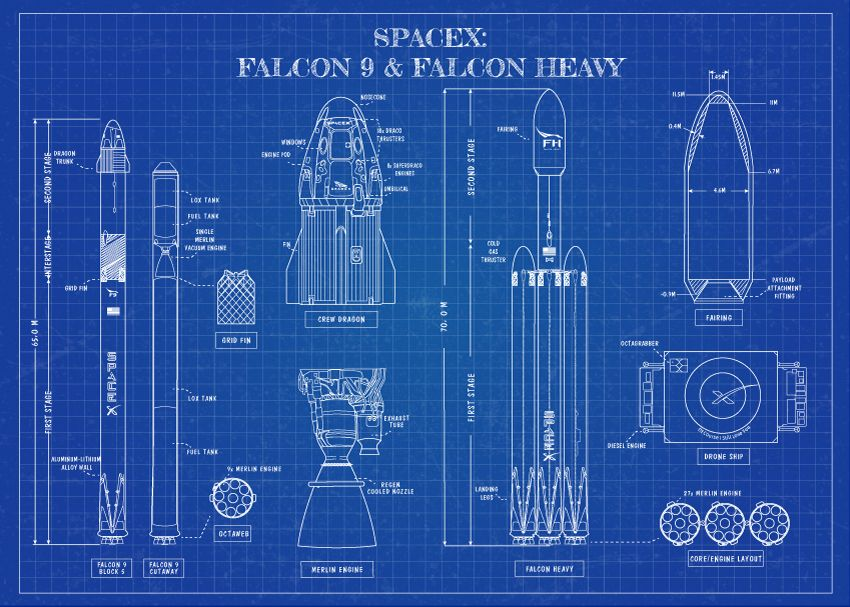
\includegraphics[width=0.4\textwidth]{gambar/cetakbiru.jpg}

  % Ubah sesuai dengan keterangan gambar yang diinginkan.
  \caption{Cetak biru roket yang akan diuji coba. \cite{cetakbiruspacex}}
  \label{fig:cetakbiru}
\end{figure}

\lipsum[9-10]

\subsection{Lorem Ipsum}
\label{subsec:loremipsum}

\lipsum[11]

% Contoh pembuatan tabel.
\begin{table}
  \caption{Contoh tabel sederhana}
  \label{tab:tabelsederhana}
  \centering
  \begin{tabular}{lll}
    \toprule
    Heading1 & Heading2 & Heading3  \\
    \midrule
    One      & Two      & Three     \\
    Four     & Five     & Six       \\
    \bottomrule
  \end{tabular}
\end{table}

% Contoh pembuatan potongan kode.
\begin{lstlisting}[
  language=C++,
  caption={Program halo dunia.},
  label={lst:halodunia}
]
#include <iostream>

int main() {
    std::cout << "Halo Dunia!";
    return 0;
}
\end{lstlisting}

\lipsum[12]

% Contoh pembuatan daftar.
\begin{enumerate}
  \item \lipsum[13][1-4]
  \item \lipsum[13][5-8]
  \item \lipsum[13][9-12]
\end{enumerate}

\lipsum[14-15]

  % Ubah judul dan label berikut sesuai dengan yang diinginkan.
\section{Lorem ipsum}
\label{sec:loremipsum}

% Ubah paragraf-paragraf pada bagian ini sesuai dengan yang diinginkan.

% Contoh input beberapa gambar pada halaman.
\begin{figure*}
  \centering
  \subfloat[Hasil A]{\includegraphics[width=.4\textwidth]{example-image-a}
    \label{fig:hasila}}
  \hfil
  \subfloat[Hasil B]{\includegraphics[width=.4\textwidth]{example-image-b}
    \label{fig:hasilb}}
  \caption{Contoh input beberapa gambar.}
  \label{fig:hasil}
\end{figure*}

\lipsum[16-18]

% Contoh input potongan kode dari file.
\lstinputlisting[
  language=Python,
  caption={Program perhitungan bilangan prima.},
  label={lst:bilanganprima}
]{program/bilangan-prima.py}

\lipsum[19-20]

  % Ubah judul dan label berikut sesuai dengan yang diinginkan.
\section{Kesimpulan}
\label{sec:kesimpulan}

% Ubah paragraf-paragraf pada bagian ini sesuai dengan yang diinginkan.

\lipsum[21-23]


  % Menampilkan daftar pustaka dengan format IEEE
  \bibliographystyle{IEEEtranN}
  \bibliography{pustaka/pustaka.bib}

  % Menyeimbangkan bagian akhir di kedua kolom
  \balance

\end{document}
